\chapter{\textbf{绪论}}%第一章
\section[\textnormal{引言}]{\textbf{引言}}

磁场重联是天体物理以及等离子体物理中非常重要的内容,在天体物理中像是太阳耀斑、磁层暴、
日冕物质抛射\cite{ANOKEUZOSIKE20244314}、$\gamma$射线暴等都可能是由磁场重连后产生的能量驱动的\cite{RevModPhys.82.603}。而在等离子体物理中,
磁场重连也是一个被广泛研究的主题。

1960年代,科学家们开始观察到太阳表面上出现的耀斑现象。
这些耀斑释放出强大的能量,并且产生了强烈的辐射,太阳表面的物质喷射甚至会影响地球上的通信和电力系统\cite{DEABREU20193586, ZHOU20244608},
但在当时科学家对耀斑的起源一直知之甚少。

之后,研究人员提出了磁场重连理论\cite{RevModPhys.82.603, Cheng_2020}来解释太阳耀斑、日冕物质抛射等太阳表面的活动现象。
在实验室等离子体中,人们开始利用磁约束聚变和等离子体装置来模拟等离子体的磁重联过程,
通过直接的实验,科学家们可以观察和验证磁重联的一些基本特征,并推动进一步的理论发展。

随着计算机技术的进步,实验室天体物理的研究开始利用数值模拟来研究磁场重连的过程,通过数值模拟\cite{Lu_2021,Yi_2018},
研究人员可以在计算机上模拟太阳等恒星的等离子体行为,并观察磁场重连的发生和演化,
这些模拟方法可以更加深入的理解磁重联的过程,并且可以验证实验观测的结果。

研究激光驱动的磁场重连是具有重要意义的科学探索,因为涉及到许多个领域的关键问题,以下是为什么这个领域重要的原因:

1. 可以了解宇宙中的一些现象,磁重联可以驱动太阳耀斑、恒星表面的活动、星际空间的等离子体运动\cite{RevModPhys.82.603}等现象。
我们可以通过研究激光驱动的磁场重连深入了解该现象背后的物理机制,加深对宇宙中磁场重连的理解。

2. 磁重联也可以在核聚变、粒子加速器\cite{Medina_Torrej_n_2023}等领域中运用。透过激光驱动的磁场重联研究,
我们可以探索有效控制和操纵等离子体的办法,从而提高聚变能量的输出效率、以及改进等离子体加热技术和加强粒子加速器的性能。

3. 由于磁场重连是太阳耀斑的能量释放过程的机制之一,也与恒星表面物质活动、抛射\cite{Lyubarsky_2001}等内容密切相关。
我们可以通过计算机模拟激光驱动的磁重联更好的理解这些现象的能量来源和能量释放的机制。

4. 因为我们是使用激光来人为触发等离子体中的磁场重联,在其中会大量使用到高能量密度的激光\cite{Takabe_Kuramitsu_2021, Yi_2018},
这可以帮助我们研究高能量密度条件下的等离子体和激光的相互作用。透过使用激光技术,
可以在受控的实验条件下模拟并驱动磁场重连,为其它研究提供数据支持。

\section[\textnormal{磁重联原理介绍}]{\textbf{磁重联原理介绍}}

磁场重联涉及磁场线重新连接并释放储存在磁场中的能量。在磁重联过程中,
原本彼此相互沿着磁力线运动的等离子体区域被重新连接在一起,导致磁场的拓扑结构发生变化。
这通常会发生在等离子体中磁场较大的区域\cite{2009ARA&A..47..291Z},例如太阳的日冕区域,地球磁层等。

一般来讲,磁重联会伴随着能量的释放和粒子加速的现象。在太阳耀斑中,
磁重联发生会出现强烈的能量耗散致使大量粒子伴随强大的电磁辐射被发射出去,并且会对地球产生影响,其具体的原理如下介绍:

1.	磁场线交错和重新连接\cite{2009ARA&A..47..291Z}: 

在磁重联发生的过程中,等离子体中的日冕区域会出现磁场线会开始出现互相交错然后重新连接。

2.	磁场能量转化\cite{GU2023100018}: 

当磁场线重新连接时,磁场能量会产生磁重联区域的局部加热,使等离子体温度升高。随着这一过程,
磁重联区域产生的磁岛结构(见图*)会导致磁场能量的释放,这样释放出来的能量可以转化为热能和粒子的动能,
从而加热等离子体和导致粒子的动能增加。进而导致等离子体中的各种现象,例如耀斑、日冕物质抛射等。

3.	Sweet-Parker模型\cite{annurev:/content/journals/10.1146/annurev-astro-082708-101726, 1958IAUS....6..123S, Yang_2019}:
Sweet-Parker模型是解释磁重联过程的经典模型之一。

Sweet-Parker模型的关键假设是等离子体中存在磁场线重联的狭窄区域,称为电流片(current sheet)(见图)。
在电流片中,磁场线由于不稳定性而发生重新连接,导致了能量释放和等离子体的加热。

Sweet-Parker模型的基本过程如下:

I. 形成电流片: 在等离子体中,由于磁场线的漂移和重排,会形成一个狭窄的区域,其中磁场线密集且方向相反,这就是电流片。

II. 磁场线重联: 在电流片中,磁场线重新连接,使得磁能转化为等离子体内部的热能和动能。这个过程会释放大量的能量,并导致等离子体的加热。

III. 能量释放: 重联过程释放的能量会导致等离子体的加热和加速。这些能量释放的过程形成了太阳耀斑和日冕物质抛射等现象。

Sweet-Parker模型的一个重要特征是它的演化过程是相对缓慢的\cite{2009ARA&A..47..291Z},而且通常是不稳定的。
这说明模型预测的重联速率相对较慢,与观测到的太阳耀斑爆发速率相比可能较慢。
因此,Sweet-Parker模型在解释一些太阳活动现象时可能存在一些局限性。

尽管如此,Sweet-Parker模型为我们理解磁场线重联的基本过程提供了一个简单而有用的框架,并且仍然是研究太阳等离子体物理的重要工具之一。

4.	Hall 重联\footnote{又称作无碰撞重连}\cite{annurev:/content/journals/10.1146/annurev-astro-082708-101726, Uzdensky_2006}:
在等离子体中,如果存在磁重联现象,即磁场线重新连接的过程,那么在这些重新连接的区域可能会产生局部的电场。
如果这些重新连接的磁场线穿过导电等离子体,那么Hall效应会导致横向电场的产生,从而形成Hall电势。
同时,在Hall重联中,磁场也会形成一个四极场模式,在观测中也可以以四极场模式的出现与否来判断Hall重联。
又因为在Hall重连中,等离子体粒子平均自由程大于系统尺寸,所以不会出现粒子碰撞的现象,故又将其称为无碰撞重联。


5. 相对论性磁重联\cite{Uzdensky_2011}:	相对论性磁重联是在磁场主导的环境中,当磁能密度远超过等离子体静质量能密度时发生的现象。
重联条件一般用磁化参数$\displaystyle\sigma=\frac{B_0^2}{4\pi nm_e c^2}$表示,即磁能密度与静质量能密度的比值大于一定阈值,或者,
磁场的能量密度远远大于等离子体的热能密度。
当$\displaystyle\sigma\gg 1$时,磁场能量占主导地位,被认为是相对论性磁场。
其中$B_0$为磁场,n是等离子体密度,$m_e$是电子质量,c是光速。相反,当$\sigma<1$等离子体的热能占主导地位,磁场的影响相对较小,
这通常被称为非相对论性磁场。

总的来说,磁重联是一种重要的磁流体现象,它不仅在太阳等天体物理现象中起着关键作用,
还在实验室等离子体中被广泛研究。通过理解磁重联的原理,人们可以更好地理解宇宙中的等离子体行为,
并且有助于解释和预测各种天体物理现象。

\section[\textnormal{磁场重连的国内外研究现状和其意义}]{\textbf{磁场重连的国内外研究现状和其意义}}

在本章的最后,我们将讨论近年来国内外各研究机构在激光等离子体磁重联领域取得的一些重要进展,并展望未来的研究方向和挑战。

在国内,国防科技大学团队于2023年发表了一篇关于激光诱导等离子体泡产生唯电子磁重联的三维例子模拟\cite{https://doi.org/10.1029/2023GL104868}的文章。
该研究揭示了唯电子磁重联这一在地球磁层中新发现的重联模式。
唯电子磁重联是指磁场能量在没有离子耦合的电子尺度电流片中被转化和耗散的现象。
该团队通过激光等离子体相互作用,在湍流等离子体中观察到了一种特殊形式的磁重联,被称为唯电子重联。

在研究中,激光与物质相互作用产生了磁泡,而重联电流片则形成在激光产生的磁泡的界面处。
随着重联的演化,电流片变窄并最终断裂,导致两个泡合并成一个细长的泡。值得注意的是,
在这个过程中,电子外流占主导地位,而离子外流则可以忽略不计。能量转换主要发生在X线附近,
而重联重联场则驱动了整个能量转换的过程。这一研究为理解激光诱导的唯电子磁重联提供了实验证据,
为相对论性磁重联的实验研究开辟了新的途径。

在国外,Matthew Goodbred\cite{PhysRevLett.129.265101}提出了一种宇宙对等等离子体中相对论磁重联速率的第一原理模型,
该模型分析表明在磁场主导的相对论区域中,x线热压力显著低于上游磁压力,这是由于维持电流密度所需的极端能量,
与动力学模拟一致。这导致上游磁力线向内坍缩,产生开放的流出几何形状,从而实现快速重联。

文章中解释了重联在磁场能量密度高于等离子体的静质量能量密度的各种天体物理环境中起着关键作用。
另外,当磁化参数很大时,相对论效应变得重要。快速重联速率对于解释极端天体物理环境中的瞬变耀斑和非热粒子特征等观测结果
非常重要\cite{RevModPhys.82.603}。

这些研究为我们理解磁场重联提供了重要的实验证据和理论基础;在未来,我们可以进一步研究激光驱动的磁重联现象,
拓展其在不同领域中的应用。

\chapter{\textbf{激光等离子体磁重联的模拟方法}}%第二章
\section[\textnormal{引言}]{\textbf{引言}}

强激光脉冲域等离子体相互作用产生强磁场,并导致了磁场的重联现象。这种现象不仅可以在实验室中观察到,
在天体物理和核聚变等领域也具有重要意义。

在本章中,我们将讨论激光等离子体磁重联的模拟方法。首先,我们将介绍本研究中重要的数值模拟技术,PIC方法。
接着将深入探讨基于PIC方法的模拟软件EPOCH\cite{Arber:2015hc},介绍其原理和算法。

最后,本文将会讲解基于EPOCH软件的等离子体模拟,介绍本研究中需要用到的理论模型和参数。
通过本章的介绍可以更好的理解激光等离子体的数值模拟方法,
从而在实验室天体物理、等离子体物理等领域中获得更多的手段分析等离子体。

\section[\textnormal{PIC模拟方法}]{\textbf{PIC模拟方法}}

在本小节中,我们先简单了解PIC(Particle In Cell)算法的知识,以便我们后续了解整个模拟过程以及实现方法。

\subsection[\textnormal{PIC模拟的基本原理和流程}]{\textbf{PIC模拟的基本原理和流程}}

PIC模拟是一种常用于等离子体物理和计算电磁学领域的数值模拟方法。
PIC模拟是基于将粒子模拟和网格求解结合在一起的计算方法。
该方法会将空间离散化为无数个网格,在每个网格点上跟踪粒子的轨迹,并同时在网格上求解偏微分方程。
其中等离子体由一组宏观粒子表示,每个宏观粒子对应于真实等离子体中的许多粒子。
因此,宏粒子的电荷和质量在数值上与 $e$ 和 $m_e$ 或 $m_p$ 不同,但运动方程与真实粒子相同\cite{Pohl_2020},
其基本思想是将等离子体系统划分为离散的粒子,这些粒子在离散的空间网格上移动,同时受到电磁场的相互作用。
通过对粒子轨迹的跟踪和电磁场的求解,以及为了计算作用在粒子上的力,将场值从网格点插值到粒子位置。
透过这些方法可以模拟等离子体系统的动态行为。

但是如果粒子数目太少或者空间网格太大,PIC模拟方法容易出现数据噪声和误差,
因此该模拟方法需要巨量的粒子以保证最终结果的精确性。
PIC方法主要分成两个部分,分别为粒子方法和网格方法,用以模拟等离子体行为。两者介绍如下:

1. 粒子方法:

粒子方法诸如SPH\footnote{光滑粒子流体}、MPS\footnote{Moving particle semi-implicit method}
以及本文需要着重讲解的PIC方法等都是需要基于拉格朗日描述的数值模拟方法。流体力学中,
拉格朗日描述是将物体的运动状态相对于物体自身的参考系来描述的,而非相对于外部观察者的参考系。
在拉格朗日描述中的动力学方程一般以物体的位置、速度、和时间的函数来表示,例如:
\begin{equation}
    \begin{aligned}
        &\displaystyle x=x\left(a,b,c,t\right), \\
        &\displaystyle u_x\ =\frac{\partial x\left(a,b,c,t\right)}{\partial t}
    \end{aligned}
\end{equation}

这类方程一般被称为运动方程。拉格朗日描述的特点是其可以针对任意形状和复杂运动的物体,并且不需要引入其他的参考系。

2.网格方法:

在网格方法中,我们的EPOCH软件是基于FDTD\footnote{Finite-Difference Time-Domain,即时域有限差分法}数值方法来模拟,
该方法应用非常广泛。我们在这个方法中关心的是使用空间和时间偏导数的中心差分近似。 
这意味着时间积分以leapfrog integration\cite{Skeel1993}进行。

FDTD方法的基本思想是将电磁场的时空变化离散化为网格上的差分方程,并通过时间步进的方式逐步更新场的数值。其推导过程如下所示:

首先,我们考虑一般的麦克斯韦方程组\cite{Meagher_2020}:
\begin{equation}
    \begin{aligned}
        &\displaystyle\nabla \cdot \mathbf{E} = \frac{\rho}{\varepsilon_0} \\
        &\displaystyle\nabla \cdot \mathbf{B} = 0 \\
        &\displaystyle\nabla \times \mathbf{E} = -\frac{\partial \mathbf{B}}{\partial t} \\
        &\displaystyle\nabla \times \mathbf{B} = \mu_0 \mathbf{J} + \mu_0 \varepsilon_0 \frac{\partial \mathbf{E}}{\partial t}
    \end{aligned}
\end{equation}


其中,$\mathbf{E}$ 和 $\mathbf{B}$ 分别代表电场和磁场,$\rho$ 是电荷密度,$\mathbf{J}$ 是电流密度,$\varepsilon_0$ 和 $\mu_0$ 分别是真空中的电介质常数和磁导率。

接着,我们对空间和时间进行离散化,将空间划分为网格,时间划分为离散的时间步长。设网格点 $(i, j, k)$ 处的电场和磁场分别为 $\mathbf{E}_{i,j,k}$ 和 $\mathbf{B}_{i,j,k}$。

在 FDTD 方法中,我们使用中心差分法对麦克斯韦方程组进行离散化。以电场的 $x$ 分量为例,麦克斯韦方程组\cite{Meagher_2020}的第三个方程可以近似为:
\begin{equation}
    \displaystyle\frac{\mathbf{E}_{i,j,k}^{n+1} - \mathbf{E}_{i,j,k}^{n}}{\Delta t} = -\frac{\mathbf{B}_{i,j+1,k}^{n+1/2} - \mathbf{B}_{i,j-1,k}^{n+1/2}}{\Delta y}
\end{equation}

其中,$n$ 表示时间步数,$\Delta t$ 和 $\Delta y$ 分别表示时间步长和网格间距。

我们可以用类似的方法将磁场的 $y$ 分量近似为:
\begin{equation}
    \displaystyle\frac{\mathbf{B}_{i,j,k}^{n+1/2} - \mathbf{B}_{i,j,k}^{n-1/2}}{\Delta t} = \frac{\mathbf{E}_{i,j,k}^{n+1} - \mathbf{E}_{i,j,k}^{n}}{\Delta y}
\end{equation}

通过以上的离散化方程,我们可以利用迭代的方式逐步更新电场和磁场在网格点上的数值,从而模拟电磁场的时空变化过程。这就是 FDTD 方法的基本原理和流程。

在PIC方法中,粒子方法和网格方法相互交互,共同驱动等离子体系统的模拟过程:

PIC代码的计算循环涉及到粒子和网格之间的相互作用。粒子按索引$p$编号,网格索引为$g$。在每个时间步中,循环经历四个阶段。

首先,粒子受到洛伦兹力的影响被推进到新的位置,这是通过积分粒子的运动方程实现的。

在第二阶段,从粒子数据中将电荷和/或电流加权到空间网格上。
这对应于将粒子的运动状态转化为周围网格点上的电磁场分布,从而对粒子施加相应的力。

接下来,在网格上积分场方程,更新网格上的电磁场分布,以反馈到粒子的运动状态中。

最后,在第四阶段,通过将新的磁场和电场插值到粒子位置,计算作用在粒子上的新力,从而更新粒子的位置和速度。

通过这种粒子和网格的交互作用,PIC方法能够全面地模拟等离子体的动态行为。
这种综合性的模拟方法使得PIC方法在等离子体物理和计算电磁学领域中\cite{graf2023finitedifference}得到了广泛的应用和发展。


\subsection[\textnormal{PIC模拟等离子体行为}]{\textbf{PIC模拟等离子体行为}}

上一小节介绍了PIC方法的构成,本节将介绍这一方法是如何描述等离子体行为的\cite{Qin_2015}。
我们考虑Vlasov-Maxwell system\cite{Pohl_2020},首先是Maxwell Equations: 
\begin{equation}
    \begin{aligned}
        &\displaystyle\nabla\cdot E=4\pi\rho ,\\
        &\displaystyle\nabla\times E=-\frac{1}{c}\frac{\partial B}{\partial t} ,\\
        &\displaystyle\nabla\cdot B=0 ,\\
        &\displaystyle\nabla\times B=\frac{1}{c}\frac{\partial E}{\partial t}+4\pi j\frac{1}{c} ,
    \end{aligned}
\end{equation}

接着我们考虑$\rho(x,t)$和$j(x,t)$
\begin{equation}
    \begin{aligned}
        &\displaystyle\rho(x,t) = \sum_l q_l\int f_l(x,p,t)\mathrm{d^3}p, \\
        &\displaystyle j(x,t) = \sum_l q_l\int f_l(x,p,t)v\mathrm{d^3}p
    \end{aligned}
\end{equation}

和Vlasov方程\cite{RevModPhys.55.403}:
\begin{equation}
    \begin{aligned}
        & \displaystyle \frac{\partial f_\alpha}{\partial t}+\mathbf{v}\cdot\nabla\mathbf{f}_\alpha+\frac{\mathbf{q}_\alpha}{\mathbf{m}_\alpha}\left(\mathbf{E}+\mathbf{v}\times\mathbf{B}\right)\cdot\frac{\partial\mathbf{f}_\alpha}{\partial\mathbf{v}}=0
    \end{aligned}
\end{equation}
针对Vlasov方程,他在相空间的轨迹会满足这个轨迹$\displaystyle \frac{\mathrm{d}}{\mathrm{d}t}f(x(t),p(t),t) = 0$,
该轨迹由如下的常微分方程给出:
\begin{equation}
    \begin{aligned}
        &\displaystyle\frac{\mathrm{d}x}{\mathrm{d}t} = v(t), \\
        &\displaystyle\frac{\mathrm{d}p}{\mathrm{d}t} = F(x(t),t)/m
    \end{aligned}
\end{equation}

这是带有洛伦兹力$\displaystyle F = q(E+\frac{1}{c}v\times B)$的相对论性运动方程,
运动方程会由于给定的初始条件$f(x,p,t) = 0$,产生一组表示像相空间表面的曲线,此即Vlasov方程的解

在真实处理场的时候,我们会使用到前述的FDTD来求解最终的电磁场(见示意图\ref{FDTD_fig}),
\begin{figure}[H]
    \centering
    \tikzset{every picture/.style={line width=0.75pt}} %set default line width to 0.75pt        

    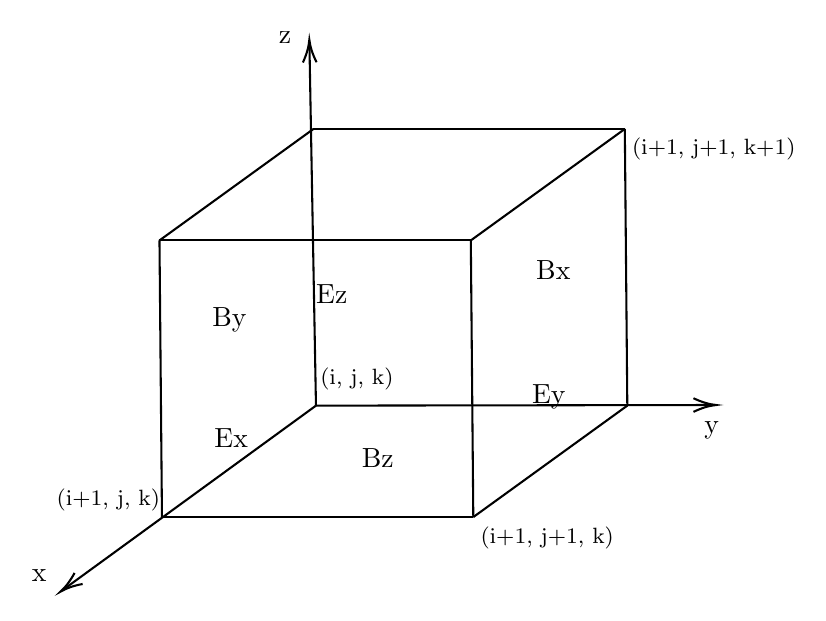
\begin{tikzpicture}[x=0.75pt,y=0.75pt,yscale=-1,xscale=1]
    %uncomment if require: \path (0,300); %set diagram left start at 0, and has height of 300
    
    %Straight Lines [id:da6034276674665278] 
    \draw    (177,115) -- (178.2,248.3) ;
    %Straight Lines [id:da655173803092191] 
    \draw    (327,115) -- (328.2,248.3) ;
    %Straight Lines [id:da3878341014241171] 
    \draw    (328.2,248.3) -- (178.2,248.3) ;
    %Straight Lines [id:da028818132460584733] 
    \draw    (327,115) -- (177,115) ;
    %Straight Lines [id:da13072090565287353] 
    \draw    (251.2,61.3) -- (177,115) ;
    %Straight Lines [id:da8697417945417365] 
    \draw    (401.2,61.3) -- (327,115) ;
    %Straight Lines [id:da8159253833700819] 
    \draw    (401.2,61.3) -- (251.2,61.3) ;
    %Straight Lines [id:da18423509429124674] 
    \draw    (401.2,61.3) -- (402.4,194.6) ;
    %Straight Lines [id:da25343219955771845] 
    \draw    (402.4,194.6) -- (328.2,248.3) ;
    %Straight Lines [id:da6310805912347262] 
    \draw    (252.4,194.6) -- (155.23,265.35) -- (130.82,283.12) ;
    \draw [shift={(129.2,284.3)}, rotate = 323.94] [color={rgb, 255:red, 0; green, 0; blue, 0 }  ][line width=0.75]    (10.93,-3.29) .. controls (6.95,-1.4) and (3.31,-0.3) .. (0,0) .. controls (3.31,0.3) and (6.95,1.4) .. (10.93,3.29)   ;
    %Straight Lines [id:da6004799236910141] 
    \draw    (252.4,194.6) -- (443.2,194.3) ;
    \draw [shift={(445.2,194.3)}, rotate = 179.91] [color={rgb, 255:red, 0; green, 0; blue, 0 }  ][line width=0.75]    (10.93,-3.29) .. controls (6.95,-1.4) and (3.31,-0.3) .. (0,0) .. controls (3.31,0.3) and (6.95,1.4) .. (10.93,3.29)   ;
    %Straight Lines [id:da8421338634253295] 
    \draw    (252.4,194.6) -- (249.24,20.3) ;
    \draw [shift={(249.2,18.3)}, rotate = 88.96] [color={rgb, 255:red, 0; green, 0; blue, 0 }  ][line width=0.75]    (10.93,-3.29) .. controls (6.95,-1.4) and (3.31,-0.3) .. (0,0) .. controls (3.31,0.3) and (6.95,1.4) .. (10.93,3.29)   ;
    
    % Text Node
    \draw (114,272) node [anchor=north west][inner sep=0.75pt]   [align=left] {x};
    % Text Node
    \draw (438,201) node [anchor=north west][inner sep=0.75pt]   [align=left] {y};
    % Text Node
    \draw (233,13) node [anchor=north west][inner sep=0.75pt]   [align=left] {z};
    % Text Node
    \draw (202,204) node [anchor=north west][inner sep=0.75pt]   [align=left] {Ex};
    % Text Node
    \draw (355,183) node [anchor=north west][inner sep=0.75pt]   [align=left] {Ey};
    % Text Node
    \draw (251,135) node [anchor=north west][inner sep=0.75pt]   [align=left] {Ez};
    % Text Node
    \draw (357,123) node [anchor=north west][inner sep=0.75pt]   [align=left] {Bx};
    % Text Node
    \draw (201,146) node [anchor=north west][inner sep=0.75pt]   [align=left] {By};
    % Text Node
    \draw (273,214) node [anchor=north west][inner sep=0.75pt]   [align=left] {Bz};
    % Text Node
    \draw (253,175) node [anchor=north west][inner sep=0.75pt]   [align=left] {{\footnotesize (i, j, k)}};
    % Text Node
    \draw (330.2,251.3) node [anchor=north west][inner sep=0.75pt]   [align=left] {{\footnotesize (i+1, j+1, k)}};
    % Text Node
    \draw (126,233) node [anchor=north west][inner sep=0.75pt]   [align=left] {{\footnotesize (i+1, j, k)}};
    % Text Node
    \draw (403.2,64.3) node [anchor=north west][inner sep=0.75pt]   [align=left] {{\footnotesize (i+1, j+1, k+1)}};
    
    
    \end{tikzpicture}
    \caption{FDTD方法示意图}
\label{FDTD_fig}
\end{figure}

这种方法应用到前述的Maxwell equations时,可以得到精确的数值结果:
\begin{equation}
    \begin{aligned}
        &\displaystyle\mathbf{E}^{n+1}=\mathbf{E}^n+c\Delta t(\nabla\times\mathbf{B})^{n+1/2}-4\pi\mathbf{j}^{n+1/2},\\
        &\displaystyle\mathbf{B}^{n+1/2}=\mathbf{B}^{n-1/2}-c\Delta t(\nabla\times\mathbf{E})^n
    \end{aligned}
\end{equation}

洛伦兹力
\begin{equation}
    \displaystyle\mathbf{F}^n=q(\mathbf{E}^n+1/2c(\mathbf{v}^{n+1/2}+\mathbf{v}^{n-1/2})\times\mathbf{B}^n)
\end{equation}

接着,我们可以根据粒子受到的洛伦兹力,利用上述的常微分方程,对粒子的位置和速度进行更新。这一步相当于将粒子在相空间中的运动轨迹推进到新的时间步长。
然后根据粒子的位置和速度,计算空间网格上的电荷密度和电流密度。这一步是将粒子的信息投影到空间网格上,用于更新电磁场。
随后,根据电荷密度和电流密度,在空间网格上求解Maxwell方程组,得到新的电场和磁场分布。这一步利用FDTD方法进行数值求解。
最后可以利用新的电场和磁场分布,对粒子受到的洛伦兹力进行计算。这一步将电场和磁场的信息插值到粒子的位置上,得到粒子在新时间步上的受力情况。

\section[\textnormal{理论模型及具体参数设置}]{\textbf{理论模型及具体参数设置}}

介绍完我们PIC模拟的基本原理,我们接下来要介绍本研究的基础实验设置。

分两个部分:其一为针对线偏振激光入射等离子体模型的参数分析;
第二部针对新参数激光(即圆偏振激光)与当前等离子体的相互作用对磁重联的影响。

1. 针对针对线偏振激光入射等离子体模型的参数\cite{Yi_2018}:
首先我们设定一个等离子体薄靶(见图\ref{plasma_taret}),
薄靶的大部分区域密度$n_c=m_e\omega_0^2/4\pi e^2=1.1\times10^{21}\mathrm{cm}^{-3}$,\\
\begin{figure}[H]
    \centering
    \tikzset{every picture/.style={line width=0.75pt}} %set default line width to 0.75pt        

    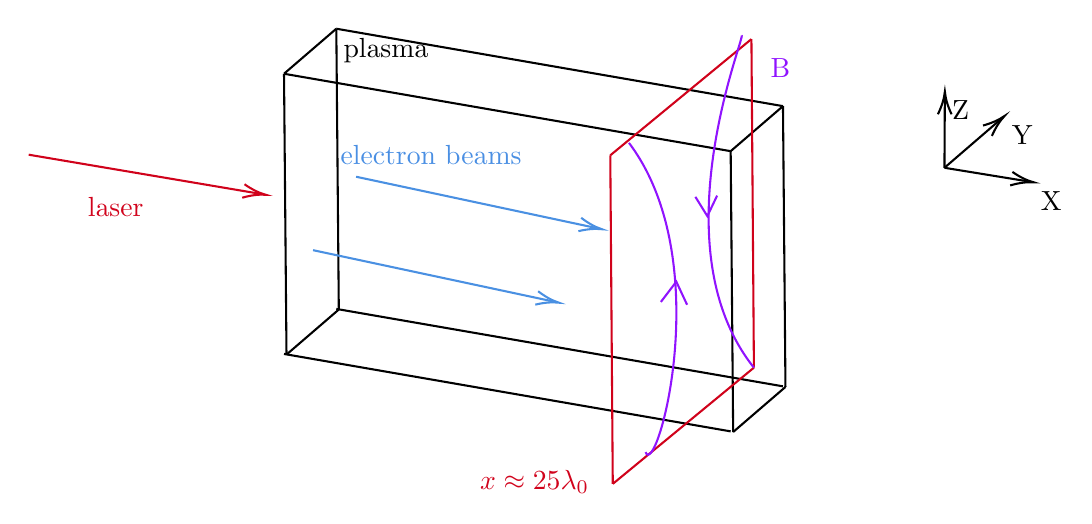
\begin{tikzpicture}[x=0.75pt,y=0.75pt,yscale=-1,xscale=1]
    %uncomment if require: \path (0,300); %set diagram left start at 0, and has height of 300
    
    %Straight Lines [id:da6973655206794538] 
    \draw    (218,79) -- (433.2,116.3) ;
    %Straight Lines [id:da19628227164037182] 
    \draw    (243.2,57.3) -- (458.4,94.6) ;
    %Straight Lines [id:da9746417463241981] 
    \draw    (218,79) -- (243.2,57.3) ;
    %Straight Lines [id:da16967524503600173] 
    \draw    (433.2,116.3) -- (458.4,94.6) ;
    %Straight Lines [id:da26458912267398427] 
    \draw    (218,79) -- (219.2,214.3) ;
    %Straight Lines [id:da9124575729970188] 
    \draw    (243.2,57.3) -- (244.4,192.6) ;
    %Straight Lines [id:da02509023758106199] 
    \draw    (433.2,116.3) -- (434.4,251.6) ;
    %Straight Lines [id:da46827733238245317] 
    \draw    (458.4,94.6) -- (459.6,229.9) ;
    %Straight Lines [id:da62662556038416] 
    \draw    (219.2,214.3) -- (244.4,192.6) ;
    %Straight Lines [id:da15715730601440026] 
    \draw    (434.4,251.6) -- (459.6,229.9) ;
    %Straight Lines [id:da7392369143868653] 
    \draw    (218,214) -- (433.2,251.3) ;
    %Straight Lines [id:da12818875758600945] 
    \draw    (243.2,192.3) -- (458.4,229.6) ;
    %Straight Lines [id:da3077997186295198] 
    \draw [color={rgb, 255:red, 208; green, 2; blue, 27 }  ,draw opacity=1 ]   (95,118) -- (207.23,136.97) ;
    \draw [shift={(209.2,137.3)}, rotate = 189.59] [color={rgb, 255:red, 208; green, 2; blue, 27 }  ,draw opacity=1 ][line width=0.75]    (10.93,-3.29) .. controls (6.95,-1.4) and (3.31,-0.3) .. (0,0) .. controls (3.31,0.3) and (6.95,1.4) .. (10.93,3.29)   ;
    %Straight Lines [id:da828903884498895] 
    \draw [color={rgb, 255:red, 74; green, 144; blue, 226 }  ,draw opacity=1 ]   (252.75,128.62) -- (369.24,153.49) ;
    \draw [shift={(371.2,153.91)}, rotate = 192.05] [color={rgb, 255:red, 74; green, 144; blue, 226 }  ,draw opacity=1 ][line width=0.75]    (10.93,-3.29) .. controls (6.95,-1.4) and (3.31,-0.3) .. (0,0) .. controls (3.31,0.3) and (6.95,1.4) .. (10.93,3.29)   ;
    %Straight Lines [id:da7128181699500584] 
    \draw [color={rgb, 255:red, 74; green, 144; blue, 226 }  ,draw opacity=1 ]   (232,164) -- (348.5,188.88) ;
    \draw [shift={(350.45,189.3)}, rotate = 192.05] [color={rgb, 255:red, 74; green, 144; blue, 226 }  ,draw opacity=1 ][line width=0.75]    (10.93,-3.29) .. controls (6.95,-1.4) and (3.31,-0.3) .. (0,0) .. controls (3.31,0.3) and (6.95,1.4) .. (10.93,3.29)   ;
    %Straight Lines [id:da37524342118620124] 
    \draw [color={rgb, 255:red, 208; green, 2; blue, 27 }  ,draw opacity=1 ]   (375.2,118.3) -- (443.2,62.3) ;
    %Straight Lines [id:da057930702641196596] 
    \draw [color={rgb, 255:red, 208; green, 2; blue, 27 }  ,draw opacity=1 ]   (375.2,118.3) -- (376.4,276.61) ;
    %Straight Lines [id:da31545793099113273] 
    \draw [color={rgb, 255:red, 208; green, 2; blue, 27 }  ,draw opacity=1 ]   (443.2,62.3) -- (444.4,220.61) ;
    %Straight Lines [id:da5618379798955881] 
    \draw [color={rgb, 255:red, 208; green, 2; blue, 27 }  ,draw opacity=1 ]   (376.4,276.61) -- (444.4,220.61) ;
    %Curve Lines [id:da6483298738415948] 
    \draw [color={rgb, 255:red, 144; green, 19; blue, 254 }  ,draw opacity=1 ]   (438.4,60.61) .. controls (441.4,58.61) and (397.4,161.61) .. (444.4,220.61) ;
    %Curve Lines [id:da4282297196907223] 
    \draw [color={rgb, 255:red, 144; green, 19; blue, 254 }  ,draw opacity=1 ]   (384.2,112.3) .. controls (427.2,169.3) and (397.2,275.3) .. (392.2,261.3) ;
    \draw  [color={rgb, 255:red, 144; green, 19; blue, 254 }  ,draw opacity=1 ] (399.57,188.94) -- (407.01,179.16) -- (412.2,190.3) ;
    \draw  [color={rgb, 255:red, 144; green, 19; blue, 254 }  ,draw opacity=1 ] (426.67,137.72) -- (421.96,147.59) -- (416.2,138.3) ;
    %Straight Lines [id:da46384218883966155] 
    \draw    (536.2,124.3) -- (577.23,130.98) ;
    \draw [shift={(579.2,131.3)}, rotate = 189.25] [color={rgb, 255:red, 0; green, 0; blue, 0 }  ][line width=0.75]    (10.93,-3.29) .. controls (6.95,-1.4) and (3.31,-0.3) .. (0,0) .. controls (3.31,0.3) and (6.95,1.4) .. (10.93,3.29)   ;
    %Straight Lines [id:da5239635922849941] 
    \draw    (536.2,124.3) -- (536.39,89.6) ;
    \draw [shift={(536.4,87.6)}, rotate = 90.31] [color={rgb, 255:red, 0; green, 0; blue, 0 }  ][line width=0.75]    (10.93,-3.29) .. controls (6.95,-1.4) and (3.31,-0.3) .. (0,0) .. controls (3.31,0.3) and (6.95,1.4) .. (10.93,3.29)   ;
    %Straight Lines [id:da7689472053585253] 
    \draw    (536.2,124.3) -- (563.69,100.61) ;
    \draw [shift={(565.2,99.3)}, rotate = 139.24] [color={rgb, 255:red, 0; green, 0; blue, 0 }  ][line width=0.75]    (10.93,-3.29) .. controls (6.95,-1.4) and (3.31,-0.3) .. (0,0) .. controls (3.31,0.3) and (6.95,1.4) .. (10.93,3.29)   ;
    
    % Text Node
    \draw (122,137) node [anchor=north west][inner sep=0.75pt]   [align=left] {\textcolor[rgb]{0.82,0.01,0.11}{laser}};
    % Text Node
    \draw (243.78,112.07) node [anchor=north west][inner sep=0.75pt]   [align=left] {\textcolor[rgb]{0.29,0.56,0.89}{electron beams}};
    % Text Node
    \draw (451,70) node [anchor=north west][inner sep=0.75pt]   [align=left] {\textcolor[rgb]{0.56,0.07,1}{B}};
    % Text Node
    \draw (581.2,134.3) node [anchor=north west][inner sep=0.75pt]   [align=left] {X};
    % Text Node
    \draw (567.2,102.3) node [anchor=north west][inner sep=0.75pt]   [align=left] {Y};
    % Text Node
    \draw (538.4,90.6) node [anchor=north west][inner sep=0.75pt]   [align=left] {Z};
    % Text Node
    \draw (245.2,60.3) node [anchor=north west][inner sep=0.75pt]   [align=left] {plasma};
    % Text Node
    \draw (311,268.4) node [anchor=north west][inner sep=0.75pt]    {$\textcolor[rgb]{0.82,0.01,0.11}{x\approx 25\lambda _{0}}$};
    
    
    \end{tikzpicture}
    \caption{等离子体薄靶设置}
    \label{plasma_taret}
\end{figure}


随着x的增加,密度出现指数下降,即$\displaystyle n=n_0exp\left(-\left(x-x_0\right)^2/2l^2\right)$,该区域也称日冕区域。
激光传播时会在等离子体两侧激发两束高能电子束,当电子束传播到密度剧烈变化的区域时,电子束不足以形成强大的回流电流,
由安培力定律导致两束电子互相靠近,由两束电子束激发的磁场线也会靠近直至发生重联。\\
\begin{figure}[H]
    \centering
    \includegraphics[width=0.5\textwidth]{figures/vertopal_Figure_1.eps}
    \caption{等离子体密度$\displaystyle n=n_0exp\left(-\left(x-x_0\right)^2/2l^2\right)$}
    \label{density_plasma}
\end{figure}


在模拟的常量部分,我们首先定义了光学参数。波长为$\lambda_0$,并透过光速c和波长计算得到角频率$\omega$。
模拟的总时间设定为$\displaystyle 25T_0 = 25\times 2\lambda_0/c$,$T_0\approx 6.6fs$,模拟的空间边界条件($x\times y\times z$)为$40\times 20\times 20$

激光的部分使用了归一化振幅$a_0 = eE_0/m_sc\omega_0 = 5$且焦斑为$4\lambda_0$的激光束,激光的脉冲时间是$\displaystyle T(t) = \sin^2(\frac{\pi t}{\tau})$
激光脉冲功率和能量分别为12TW和200mJ,激光采用三维高斯分布函数且为线偏振激光(y方向偏振)。

在等离子体参数部分,需要考虑粒子的种类和他们的密度。
对于粒子种类的定义,我们分别设定了5个电子和3个质子。表明这是一个非均匀的等离子体;
定义完粒子种类之后需要定义等离子体的总共的密度,我们考虑等离子体临界密度$n_c=m_e\omega_0^2/4\pi e^2=1.1\times10^{21}\mathrm{cm}^{-3}$。
考虑到实验设置需要区分日冕区域\footnote{即重联发生的区域},所以需要将两者密度区分开来,因此在非日冕区的大部分区域等离子体密度都是取$n_0 = 20n_c$
在日冕区域$\displaystyle n=n_0exp\left(-\left(x-x_0\right)^2/2l^2\right)$出现密度剧烈变化来触发磁重联

接着,等离子体板尺寸(xyz)为$20\lambda_0\times 1\lambda_0 \times 10\lambda_0$,等离子体的初始温度为1KeV。

在模拟的网格选取中,我们选择了三维的网格$800\times 400\times 400$的网格以得到结果,
说明我们的模拟被分割成的$800\times 400\times 400$的小方块。
这样的网格设置会影响我们对等离子体与激光相互作用过程的精细度和准确性。
较高的分辨率使得我们能够更细致地观察模拟中的物理现象,但也增加了计算的复杂性和资源需求。
通过这个网格,我们可以捕捉到空间中细小尺度的变化,有助于模拟更真实和详细的物理过程。

最后,输出设置定义了在模拟过程中输出的频率和输出的数据类型,包括网格属性、重联场、磁场、电流、粒子分布等。
这样就可以在一份档案内读取不同标签的数据。

2. 针对新参数激光与当前等离子体的相互作用

在这一部分,我们需要修改激光参数尝试以不同的方法观察激光入射等离子体后产生的激光等离子体相互作用。
在上一个部分使用了线偏振激光来入射等离子体。在这一部分考虑使用圆偏振激光入射等离子体观察其相互作用。

这里圆偏振激光考虑使用两束线偏激光透过不同相位和偏振方向组合而成,旨在考虑不同激光入射对等离子体的不同影响,
以及磁重联是否会发生。
\begin{comment}
\section[\textnormal{激光等离子体相互作用}]{\textbf{激光等离子体相互作用}}

1. 首先考虑线偏振激光入射后的等离子体行为:
我们考虑到该实验是需要人为触发磁场重联现象,激光入射等离子体后,会有

激光等离子体相互作用过程描述:
在这一部分,你可以介绍激光与等离子体相互作用的基本过程,包括激光入射后与等离子体的相互作用方式,可能产生的等离子体反应等。你可以详细描述激光的传播、吸收和散射过程,以及激光能量如何转化为等离子体动能等方面的情况。

影响参数及实验设置:
在这一部分,你可以介绍不同参数设置下激光等离子体相互作用的影响。包括激光参数的变化如何影响等离子体的响应,以及不同实验条件下可能产生的物理效应。你可以列举不同参数设置的方案,并讨论其可能的影响和预期的结果。

激光等离子体相互作用的物理效应:
在这一部分,你可以详细描述激光与等离子体相互作用可能产生的物理效应。这些效应可能包括等离子体的加热、加速、激发等,以及激光与等离子体相互作用后可能产生的等离子体波动、磁重联等现象。

2. 接着考虑圆偏振激光入射后的等离子体行为:

在圆偏振激光的情况中,我们设置的是

\end{comment}

\chapter{\textbf{线偏振激光下模拟结果分析}}

\section[\textnormal{引言}]{\textbf{引言}}

在本章中,我们将会讨论一般线激光入射等离子体薄靶之后的现象,
第一个部分,本文会首先讨论模拟中磁重联发生的过程,分析模拟结果中电场和磁场的变化。
在重联过程中,根据不同的激光和等离子体条件,也会有不同的重联模型\cite{2009ARA&A..47..291Z},比如相对论性判断($\beta>1$或$\beta<1$),
重联速率,和粒子碰撞等。除此之外,磁场结构模式的不同以及其对应的理论基础,并由此推导知道磁重联的不同模式;
再者,也可以透过对重联场的研究尝试得到磁场重联的重联率,这对了解区分不同模式的重联也非常重要。%接着,磁场的在拓扑结构变化时也会针对磁场线的受力分析以及其在本研究中的重要性。

第二个部分会讨论到磁场重联一个非常重要的部分,即磁场能量转移和粒子出射现象。
天体物理中观测到的磁重联有很大的部分是和粒子射流相关,在磁重联的过程中,
随着磁场拓扑结构的变化,磁场中的能量也会接着释放。

\section[\textnormal{数值模拟结果}]{\textbf{数值模拟结果}}

\subsection[\textnormal{磁重联过程}]{\textbf{磁重联过程}}

对于磁场重联,我们在本文中会希望关注相对论性磁重联,
即$\displaystyle\sigma=\frac{B_0^2}{4\pi nme c^2}\gg 1$的磁能占主导地位的情况。
与此同时,我们的研究需要关注的是空间等离子体测量和天文观测中会需要的低$\beta$环境,
亦即$\displaystyle\beta = \frac{2\mu_0nk_BT}{B^2}<1$\cite{10.1063/1.3694119}的情况。本文中两者都是磁能占主导的模式。

上式中$\mu_0$是真空磁导率,n 是等离子体密度,$k_B$是玻尔兹曼常数,T是等离子体温度,B是磁场强度。

Beta 参数是衡量等离子体的热效应对磁场的影响程度的重要指标。当$\beta$较小时,磁场压力占主导地位,
等离子体可以被认为是磁场“刚性”或“冰冷”的,而当$\beta$较大时,等离子体的热效应变得显著,磁场对等离子体的约束作用较弱。
在等离子体物理中,通常将$\beta$参数分为低$\beta$(小于 1)、中$\beta$(1 到几十)、
高$\beta$(几十到几百)和极高$\beta$(大于 1000)等范围。

在本文中,我们参考上海交通大学李政道学者易龙卿博士\cite{Yi_2018}提出的,
利用激光与微尺度等离子体板的相互作用以突破限制\cite{10.1063/1.3694119},从而可以使得我们的研究可以同时达到$\displaystyle\sigma=\frac{B_0^2}{4\pi nme c^2}\gg 1$
和$\displaystyle\beta = \frac{2\mu_0nk_BT}{B^2} <1$的状态。

磁重联的简单过程:
激光以$+x$方向传播,y方向偏振入射等离子体薄板后引起了靶面上两侧出现域激光同向传播的电子束,
电子束会引发磁场,在密度变化剧烈的区域由于实验设置,在$x=21\mu m$的区域等离子体的密度开始减小,
导致等离子体中的电子不足以维持两束电子束继续维持平行传播,
从而两束电子束因为Ampère's force law而汇聚到一起\cite{Yi_2018}。
而随着电子束反向的电流形成的磁场线也会因此被推向一起并挤压,从而引发磁重联

以上是根据实验设置得到的磁重联的发生过程,接下来我们会需要关注重联发生过程中一些比较微观的内容:

1. 在研究模拟结果时,可以看到模拟结果的横向切面(见图\ref{fig:combinedEx})上的结果,
可以发现随着激光的传播,等离子体受到了激光的能量输入,导致了等离子体内部的物理状态发生了变化。
在横向切面上,我们可以观察到电场、磁场等参数的分布情况。在激光作用的区域,
等离子体的电场发生了显著变化,形成了波动的结构。同时,由于激光与等离子体相互作用,
可能会产生局部的温度升高或降低的现象,导致温度分布不均匀。此外,磁场也会受到激光作用的影响,
可能会出现局部磁场增强或减弱的情况。当然,本文主要会关注日冕区域\footnote{即重联区,本文之后都以日冕区域称呼}的电磁场变化,以及其对应磁重联的影响。

2. 在模拟结果里(图\ref{fig:combinedB}),我们可以看到磁场在日冕区域的分布呈现一种四极形式的分布,这说明有Hall重联的现象产生,
即在磁重联的过程中,Hall效应起到了重要作用。Hall效应在这里是等离子体中的电流受到磁场和电场的共同作用而产生的现象。
在磁重联中,由于电子和离子的质量差异,电子的运动速度比离子快,导致了电子和离子之间的摩擦力不平衡。
这种不平衡会产生Hall电流,从而形成Hall磁场。Hall磁场的作用是改变磁重联区域的磁场拓扑结构,进而影响磁重联的速率和效率。

在模拟结果中观察到的四极形式的磁场分布是Hall重联的典型特征之一\cite{TREUMANN2006101, Zhang_2023},它表明在磁重联过程中,
Hall效应对磁场的影响不能被忽略。因此,在研究磁重联时,需要考虑Hall效应对磁场和等离子体的影响。

3. 反平行重联\footnote{antiparallel reconnection}:由图\ref{plasma_taret}中紫色线所表示的磁场线可以看出,反平行重联即磁场线方向一正一反的磁重联模式,本文中主要探讨的也是该模式。
在一些研究中\cite{Xu2016-jj, gonzalez2016magnetic},平行磁场重联的模拟里,磁场线未发生重联,拓扑结构保持不变。
\begin{figure}[H]
    \begin{minipage}[t]{0.5\linewidth}
        \centering
        \tikzset{every picture/.style={line width=0.75pt}} %set default line width to 0.75pt        

        \begin{tikzpicture}[x=0.75pt,y=0.75pt,yscale=-1,xscale=1]
        %uncomment if require: \path (0,300); %set diagram left start at 0, and has height of 300

        %Curve Lines [id:da527012594321129] 
        \draw    (240,41.3) .. controls (246.2,37.3) and (307.2,152.3) .. (240,254.3) ;
        %Curve Lines [id:da8651426241379772] 
        \draw    (380,40) .. controls (389.2,42.3) and (311.2,121.3) .. (380,254.3) ;
        \draw   (278.78,147.3) -- (271.19,165.52) -- (262.56,147.77) ;
        \draw   (360.59,146.74) -- (352.75,166.14) -- (341.35,148.6) ;

        \end{tikzpicture}

        \label{fig:parallel:a}
    \end{minipage}%
    \begin{minipage}[t]{0.5\linewidth}
        \centering
        \tikzset{every picture/.style={line width=0.75pt}} %set default line width to 0.75pt        

        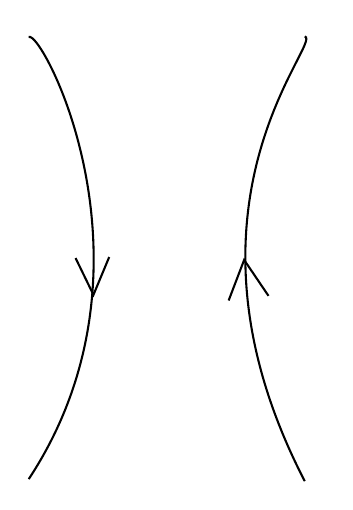
\begin{tikzpicture}[x=0.75pt,y=0.75pt,yscale=-1,xscale=1]
        %uncomment if require: \path (0,300); %set diagram left start at 0, and has height of 300
        
        %Curve Lines [id:da4272748813377649] 
        \draw    (254,52.3) .. controls (260.2,48.3) and (321.2,163.3) .. (254,265.3) ;
        %Curve Lines [id:da0467142319901368] 
        \draw    (387,52) .. controls (396.2,54.3) and (318.2,133.3) .. (387,266.3) ;
        \draw   (292.78,158.3) -- (285.19,176.52) -- (276.56,158.77) ;
        \draw   (350.33,179.23) -- (357.79,159.69) -- (369.53,177.01) ;
  
        \end{tikzpicture}
        \label{fig:antiparallel:b}
    \end{minipage}

    \caption{磁场平行与反平行示意图}
    \label{fig:combined_antiparallel}

\end{figure}


4. 研究结果时,我们可以发现在磁重联发生后会出现粒子的射流,这是因为重联过程中磁场的能量转移到等离子体热能和粒子的动能导致的,
这是磁重联发生后的一个非常重要的现象,文章将会讨论其详细过程和发生原因。

5. 在磁重联过程中,电子和离子在磁场作用下表现出不同的行为。由于电子具有较小的质量,
它们可以沿着磁力线自由移动,而不受到太多的束缚。相反,离子由于较大的质量,受到磁场的约束较为严格,
无法像电子那样自由移动。\label{idredr1}

这种电子和离子在磁场中的不同行为导致了它们在磁重联过程中的运动分离现象。具体来讲,
当磁场发生重新连接时,电子和离子会因为他们各自活跃的程度,导致它们在空间中分布不均匀。
在重新连接区域附近,电子的运动更为活跃,形成了\cite{2016ASSL..427.....G}电子扩散区\footnote{Electron Dissipation Region,下文皆称其为EDR},
而在EDR的外面一部份区域,离子受到磁场束缚,无法像电子那样移动,形成了\cite{2016ASSL..427.....G}离子扩散区\footnote{Ion Dissipation Region,下文皆称其为IDR}。

因此,EDR和IDR是在磁重联过程中形成的两个不同的区域,它们分别反映了电子和离子在磁场重新连接过程中的行为特征。
这种电子和离子的运动分离现象对于理解磁重联的动力学行为和能量释放机制具有重要意义,同时,对于研究磁场能量转移的模型也有重要的影响。

\subsection[\textnormal{电场及磁场变化}]{\textbf{电场及磁场变化}}

本小节中,我们会观察有关日冕区域的电场和磁场切片以详细的解释磁重联发生时的有关现象。\label{EB_field}

首先,我们需要先确认重联发生的区域约在哪个位置,可以由磁重联发生时的场强变化的区域来判断重联发生的区域:

\begin{figure}[H]
    \begin{minipage}[t]{0.5\linewidth}
        \centering
        \includegraphics[scale=0.2]{figures/ex14_heng.jpg}
        \label{fig:sideEx:a}
    \end{minipage}%
    \begin{minipage}[t]{0.5\linewidth}
        \centering
        \includegraphics[scale=0.2]{figures/ex15_heng.jpg}
        \label{fig:sideEx:b}
    \end{minipage}
    \begin{minipage}[t]{0.5\linewidth}
        \centering
        \includegraphics[scale=0.2]{figures/ex16_heng.jpg}
        \label{fig:sideEx:c}
    \end{minipage}%
    \begin{minipage}[t]{0.5\linewidth}
        \centering
        \includegraphics[scale=0.2]{figures/ex17_heng.jpg}
        \label{fig:sideEx:d}
    \end{minipage}
    \caption{$E_x$电场切面,可观察随着激光传播,等离子体在$x\approx 25$的区域会有场强的变化,可以由此确定重联发生的位置}
    \label{fig:combinedEx}

\end{figure}

由前述的磁重联理论中可以知道,随着重联的发生,重联场在磁重联的区域也会出现较大的变化,我们可以透过这样的特征来更好的判断磁重联发生的区域
从而定位我们需要分析的区域做分析。

接着来看电场的分布,我们主要关注电场$E_y$分量:
\begin{figure}[H]
    \begin{minipage}[t]{0.5\linewidth}
        \centering
        \includegraphics[scale=0.2]{figures/ey16xy.jpg}
        \label{fig:sideeyxy:a}
    \end{minipage}%
    \begin{minipage}[t]{0.5\linewidth}
        \centering
        \includegraphics[scale=0.2]{figures/ey17xy.jpg}
        \label{fig:sideeyxy:b}
    \end{minipage}
    \begin{minipage}[t]{0.5\linewidth}
        \centering
        \includegraphics[scale=0.2]{figures/ey18xy.jpg}
        \label{fig:sideeyxy:c}
    \end{minipage}%
    \begin{minipage}[t]{0.5\linewidth}
        \centering
        \includegraphics[scale=0.2]{figures/ey19xy.jpg}
        \label{fig:sideeyxy:d}
    \end{minipage}
    \caption{Ey电场切面,可观察到等离子体和激光传播}
    \label{fig:combined}

\end{figure}

可以看到激光沿着x方向传播的同时与等离子体相互作用,在等离子体靶的两侧边界处可以看到一正一负大小接近的场,
是因为等离子体在受到强激光入射后引起的电子等离子体振荡\cite{1923Sci....58..290L},其频率为$\omega_{pe} = \sqrt{n_e e^2/m_e \varepsilon_0}$。

接着在这个振荡层的外面可以看到电场的一个向外扩展的区域,这个区域具有波传播的特征,即类似波前的条纹斑,
每一条的间隔都是$1\mu m$。因为这些条纹基本是随着激光传播的,可以将其视为等离子体波。

接着可以看到图\ref{fig:sideeyxy:a}上的$x\approx 25$的区域,可以由此观察Ey的横切面:

\begin{figure}[H]
    \centering
    \includegraphics[width=0.5\textwidth]{figures/ey16x500.jpg}
    \caption{Ey电场横切面}
    \label{ey16_heng}
\end{figure}

上面的结果显示出:

1. 在 $x \approx 25$ 处的电场横切面呈现出一致的特征,即与激光传播方向一致,

2. 激光与等离子体的相互作用会生成电场扩展区域,这一区域呈现出向外扩展的特征,
类似于波前的条纹斑,每一条的间隔约为 $1 \mu m$。

3. 在横切面上可以看到周期相间的场强分布,这是由于电场波的传播导致的。
这些特征与振荡层内部的物理过程相符,进一步验证了电场的传播和振荡层内部物理过程之间的密切关联。



重联电场的作用:重联电场是重联率的表征量,在重联的快速增长阶段,其分布形状大致呈圆形,覆盖了电子扩散区和磁力线堆积区,其圆心位于X点附近。


接着我们来看磁场的部分,磁场横向切面的分析。在日冕区域可以观察磁场的行为

\begin{figure}[H]
    \begin{minipage}[t]{0.5\linewidth}
        \centering
        \includegraphics[scale=0.2]{figures/bx16x500.jpg}
        \label{fig:sideB:a}
    \end{minipage}%
    \begin{minipage}[t]{0.5\linewidth}
        \centering
        \includegraphics[scale=0.2]{figures/bx17x500.jpg}
        \label{fig:sideB:b}
    \end{minipage}
    \begin{minipage}[t]{0.5\linewidth}
        \centering
        \includegraphics[scale=0.2]{figures/bx18x500.jpg}
        \label{fig:sideB:c}
    \end{minipage}%
    \begin{minipage}[t]{0.5\linewidth}
        \centering
        \includegraphics[scale=0.2]{figures/bx19x500.jpg}
        \label{fig:sideB:d}
    \end{minipage}
    \caption{Bx磁场切面,可观察到四极场分布}
    \label{fig:combinedB}

\end{figure}


可以看到,随着时间的推进,重联区域的磁场逐渐出现四极形式的场分布。这一现象的出现是由于磁场在重联的过程中出现的Hall效应,
从而形成了Hall重连现象。Hall效应导致了磁场的特殊分布,其中磁场呈现出四极形式。
在下一个小节将会针对性的探讨Hall重联现象。

\subsection[\textnormal{Hall 重联现象}]{\textbf{Hall 重联现象}}

1. 发生条件:在等离子体中,如果存在磁重联现象,即磁场线重新连接的过程,那么在这些重新连接的区域可能会产生局部的电场。
如果这些重新连接的磁场线穿过导电等离子体,那么Hall效应会导致横向电场的产生,从而形成Hall电势。

等离子体和磁场如果流入离子扩散区,那么它们会和磁场的湮灭以及流出的等离子体之间保持平衡,
模拟表明\cite{10.1063/1.1597494},在没有新的等离子体输入时,重联区域的X线会沿着磁场线方向拉伸,使得这个区域的等离子体变薄。
所以,当粒子流入速度变慢的时候,会出现爆发性规模的快速无碰撞磁重联,然后将粒子从重联区域射出;
当粒子流入速度变快时,它会使电流片变宽,直到电流片宽度大于离子惯性长度,那么这时候重联速度就会减慢。然后接续上面的情况反复循环。
\begin{comment}
    由Syrovatskii的数值模拟结果表明\cite{1981ARA&A..19..163S, TREUMANN2006101},在这种情况下的电流片相对于一般的重联状况是稳定的,且不受Hall效应的影响。因此,
Hall效应对等离子体磁重联的重要性只取决于电流片的宽度,在电流片宽度$d\simeq \lambda_i$的电流片中才会出现Hall效应的重联。
\end{comment}

2. 现象观察

随着磁场重联的发生(见图\ref{fig:combinedB}),可以见到四极磁场的模式\cite{TREUMANN2006101,Yi_2018},这显示了Hall效应样式的重联接。
在重联平面内形成了沿着磁场线内侧的磁力线流向X点。
由图\ref{reconnect_cross_section}可以见得,正中间的长方形为重连的EDR,EDR外和外磁场线包围的“剩下的”区域为IDR,
在IDR区域向内的一对箭头则是Hall电场$E_y$,这也是为什么我们在\ref{fig:combined}中研究$E_y$的原因,研究它可以比较直观的看到电场分布的情况。

在IDR中,离子的整体运动很小,而电子则继续向磁层外流动,
因此由于 $\mathbf{J}=q_in\mathbf{v}i-en\mathbf{v}\epsilon$ 在离子耗散区域存在一个朝着磁层外流动的净电流。
这个电流密度产生了垂直于平面的磁场\cite{https://doi.org/10.1029/JA084iA02p00399},
根据安培定律,这个电流与包围它的磁场相关联,
右上角和左下角指向页面外,右下角和左上角指向页面内。这个具有四极结构的垂直于平面的磁场被称为霍尔磁场。
在磁层中观察到霍尔磁场的现象是无碰撞重连的关键的特征。


\begin{figure}[H]
    \centering
    \tikzset{every picture/.style={line width=0.75pt}} %set default line width to 0.75pt        

    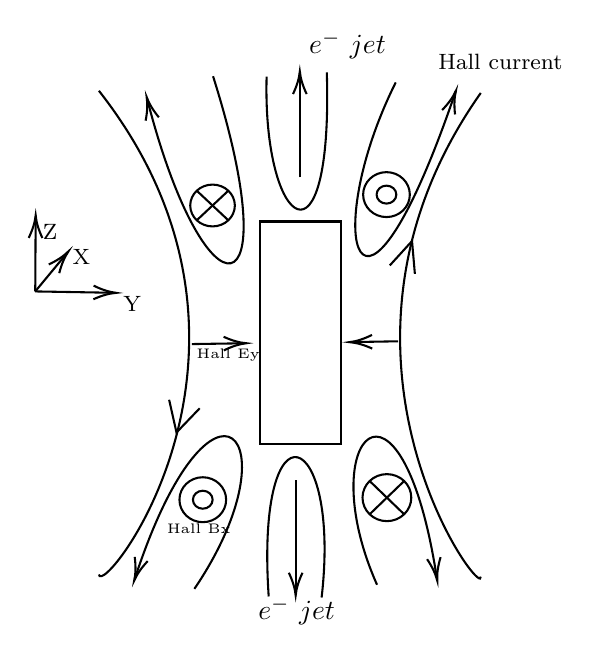
\begin{tikzpicture}[x=0.75pt,y=0.75pt,yscale=-1,xscale=1]
    %uncomment if require: \path (0,338); %set diagram left start at 0, and has height of 338
    
    %Curve Lines [id:da48323297733043824] 
    \draw    (223.87,50.63) .. controls (321.04,174.5) and (225.16,296.27) .. (223.87,283.68) ;
    %Curve Lines [id:da48145401760589657] 
    \draw    (407.85,51.68) .. controls (384.82,84.33) and (373.92,116.7) .. (370.36,146.47) .. controls (360.29,230.6) and (408.81,294.03) .. (407.85,284.73) ;
    %Shape: Rectangle [id:dp7686996309276799] 
    \draw   (301.35,113.62) -- (340.48,113.62) -- (340.48,220.69) -- (301.35,220.69) -- cycle ;
    %Curve Lines [id:da009097792982276864] 
    \draw    (366.87,46.63) .. controls (329.87,120.63) and (348.87,188.63) .. (395.87,50.63) ;
    \draw [shift={(395.87,50.63)}, rotate = 108.81] [color={rgb, 255:red, 0; green, 0; blue, 0 }  ][line width=0.75]    (10.93,-3.29) .. controls (6.95,-1.4) and (3.31,-0.3) .. (0,0) .. controls (3.31,0.3) and (6.95,1.4) .. (10.93,3.29)   ;
    %Curve Lines [id:da7569758360246022] 
    \draw    (278.87,43.63) .. controls (315.68,160.05) and (275.27,163.6) .. (247.29,55.27) ;
    \draw [shift={(246.87,53.63)}, rotate = 75.72] [color={rgb, 255:red, 0; green, 0; blue, 0 }  ][line width=0.75]    (10.93,-3.29) .. controls (6.95,-1.4) and (3.31,-0.3) .. (0,0) .. controls (3.31,0.3) and (6.95,1.4) .. (10.93,3.29)   ;
    %Curve Lines [id:da06071897699960749] 
    \draw    (269.87,290.63) .. controls (319.62,217) and (278.28,173.07) .. (241.42,284.94) ;
    \draw [shift={(240.87,286.63)}, rotate = 287.98] [color={rgb, 255:red, 0; green, 0; blue, 0 }  ][line width=0.75]    (10.93,-3.29) .. controls (6.95,-1.4) and (3.31,-0.3) .. (0,0) .. controls (3.31,0.3) and (6.95,1.4) .. (10.93,3.29)   ;
    %Curve Lines [id:da7035242269674511] 
    \draw    (357.87,288.63) .. controls (326.03,216.99) and (369.43,174.06) .. (386.61,284.95) ;
    \draw [shift={(386.87,286.63)}, rotate = 261.44] [color={rgb, 255:red, 0; green, 0; blue, 0 }  ][line width=0.75]    (10.93,-3.29) .. controls (6.95,-1.4) and (3.31,-0.3) .. (0,0) .. controls (3.31,0.3) and (6.95,1.4) .. (10.93,3.29)   ;
    %Flowchart: Summing Junction [id:dp4313333309183207] 
    \draw   (267.87,105.91) .. controls (267.87,100.34) and (272.68,95.83) .. (278.62,95.83) .. controls (284.55,95.83) and (289.37,100.34) .. (289.37,105.91) .. controls (289.37,111.47) and (284.55,115.98) .. (278.62,115.98) .. controls (272.68,115.98) and (267.87,111.47) .. (267.87,105.91) -- cycle ; \draw   (271.02,98.78) -- (286.22,113.03) ; \draw   (286.22,98.78) -- (271.02,113.03) ;
    %Flowchart: Summing Junction [id:dp5244689001643144] 
    \draw   (350.87,246.66) .. controls (350.87,240.4) and (356.13,235.33) .. (362.62,235.33) .. controls (369.11,235.33) and (374.37,240.4) .. (374.37,246.66) .. controls (374.37,252.91) and (369.11,257.98) .. (362.62,257.98) .. controls (356.13,257.98) and (350.87,252.91) .. (350.87,246.66) -- cycle ; \draw   (354.31,238.65) -- (370.93,254.67) ; \draw   (370.93,238.65) -- (354.31,254.67) ;
    %Shape: Donut [id:dp24273032973492104] 
    \draw   (357.66,100.66) .. controls (357.66,98.27) and (359.79,96.33) .. (362.42,96.33) .. controls (365.04,96.33) and (367.17,98.27) .. (367.17,100.66) .. controls (367.17,103.05) and (365.04,104.99) .. (362.42,104.99) .. controls (359.79,104.99) and (357.66,103.05) .. (357.66,100.66)(351.17,100.66) .. controls (351.17,94.68) and (356.2,89.83) .. (362.42,89.83) .. controls (368.63,89.83) and (373.67,94.68) .. (373.67,100.66) .. controls (373.67,106.64) and (368.63,111.48) .. (362.42,111.48) .. controls (356.2,111.48) and (351.17,106.64) .. (351.17,100.66) ;
    %Shape: Donut [id:dp5018283498511262] 
    \draw   (269.16,247.66) .. controls (269.16,245.27) and (271.29,243.33) .. (273.92,243.33) .. controls (276.54,243.33) and (278.67,245.27) .. (278.67,247.66) .. controls (278.67,250.05) and (276.54,251.99) .. (273.92,251.99) .. controls (271.29,251.99) and (269.16,250.05) .. (269.16,247.66)(262.67,247.66) .. controls (262.67,241.68) and (267.7,236.83) .. (273.92,236.83) .. controls (280.13,236.83) and (285.17,241.68) .. (285.17,247.66) .. controls (285.17,253.64) and (280.13,258.48) .. (273.92,258.48) .. controls (267.7,258.48) and (262.67,253.64) .. (262.67,247.66) ;
    %Straight Lines [id:da8405097778514081] 
    \draw    (318.67,238.33) -- (318.67,291.78) ;
    \draw [shift={(318.67,293.78)}, rotate = 270] [color={rgb, 255:red, 0; green, 0; blue, 0 }  ][line width=0.75]    (10.93,-3.29) .. controls (6.95,-1.4) and (3.31,-0.3) .. (0,0) .. controls (3.31,0.3) and (6.95,1.4) .. (10.93,3.29)   ;
    %Curve Lines [id:da1273324589984952] 
    \draw    (305.67,294.28) .. controls (299.17,197.28) and (340.67,212.28) .. (331.17,294.78) ;
    %Straight Lines [id:da5675650016597387] 
    \draw    (320.67,92.38) -- (320.67,43.28) ;
    \draw [shift={(320.67,41.28)}, rotate = 90] [color={rgb, 255:red, 0; green, 0; blue, 0 }  ][line width=0.75]    (10.93,-3.29) .. controls (6.95,-1.4) and (3.31,-0.3) .. (0,0) .. controls (3.31,0.3) and (6.95,1.4) .. (10.93,3.29)   ;
    %Curve Lines [id:da8039128203052084] 
    \draw    (304.67,43.78) .. controls (302.67,117.28) and (336.67,141.28) .. (333.67,41.78) ;
    %Straight Lines [id:da4541491512880813] 
    \draw    (268.67,172.67) -- (292.93,172.3) ;
    \draw [shift={(294.93,172.27)}, rotate = 179.13] [color={rgb, 255:red, 0; green, 0; blue, 0 }  ][line width=0.75]    (10.93,-3.29) .. controls (6.95,-1.4) and (3.31,-0.3) .. (0,0) .. controls (3.31,0.3) and (6.95,1.4) .. (10.93,3.29)   ;
    %Straight Lines [id:da7265038531434131] 
    \draw    (368,171.33) -- (346.57,171.7) ;
    \draw [shift={(344.57,171.74)}, rotate = 359.02] [color={rgb, 255:red, 0; green, 0; blue, 0 }  ][line width=0.75]    (10.93,-3.29) .. controls (6.95,-1.4) and (3.31,-0.3) .. (0,0) .. controls (3.31,0.3) and (6.95,1.4) .. (10.93,3.29)   ;
    %Straight Lines [id:da49539526071555806] 
    \draw    (193.2,147.3) -- (230.2,147.95) ;
    \draw [shift={(232.2,147.99)}, rotate = 181.01] [color={rgb, 255:red, 0; green, 0; blue, 0 }  ][line width=0.75]    (10.93,-3.29) .. controls (6.95,-1.4) and (3.31,-0.3) .. (0,0) .. controls (3.31,0.3) and (6.95,1.4) .. (10.93,3.29)   ;
    %Straight Lines [id:da14093049137857494] 
    \draw    (193.2,147.3) -- (193.39,112.6) ;
    \draw [shift={(193.4,110.6)}, rotate = 90.31] [color={rgb, 255:red, 0; green, 0; blue, 0 }  ][line width=0.75]    (10.93,-3.29) .. controls (6.95,-1.4) and (3.31,-0.3) .. (0,0) .. controls (3.31,0.3) and (6.95,1.4) .. (10.93,3.29)   ;
    %Straight Lines [id:da8298958012348723] 
    \draw    (193.2,147.3) -- (207.92,129.53) ;
    \draw [shift={(209.2,127.99)}, rotate = 129.64] [color={rgb, 255:red, 0; green, 0; blue, 0 }  ][line width=0.75]    (10.93,-3.29) .. controls (6.95,-1.4) and (3.31,-0.3) .. (0,0) .. controls (3.31,0.3) and (6.95,1.4) .. (10.93,3.29)   ;
    \draw   (272.45,203.59) -- (261.25,215.26) -- (257.7,199.49) ;
    \draw   (364.03,134.77) -- (374.73,123.03) -- (376.1,138.85) ;
    
    % Text Node
    \draw (323.67,20.73) node [anchor=north west][inner sep=0.75pt]    {$e^{-} \ jet$};
    % Text Node
    \draw (299.17,293.37) node [anchor=north west][inner sep=0.75pt]    {$e^{-} \ jet$};
    % Text Node
    \draw (385.9,31.48) node [anchor=north west][inner sep=0.75pt]   [align=left] {{\footnotesize Hall current}};
    % Text Node
    \draw (269.49,173.34) node [anchor=north west][inner sep=0.75pt]   [align=left] {{\tiny Hall Ey}};
    % Text Node
    \draw (209.72,125.47) node [anchor=north west][inner sep=0.75pt]  [rotate=-0.15] [align=left] {{\footnotesize X}};
    % Text Node
    \draw (234.2,147.99) node [anchor=north west][inner sep=0.75pt]   [align=left] {{\footnotesize Y}};
    % Text Node
    \draw (195.4,113.6) node [anchor=north west][inner sep=0.75pt]   [align=left] {{\footnotesize Z}};
    % Text Node
    \draw (255.2,257.84) node [anchor=north west][inner sep=0.75pt]   [align=left] {{\tiny Hall Bx}};
    
    
    \end{tikzpicture}
    \caption{重联截面示意图}
\label{reconnect_cross_section}

\end{figure}


\section[\textnormal{粒子射流}]{\textbf{粒子射流}}

在模拟结果中,可以看到日冕区域,磁场线被推在一起,导致磁场的重联。观察到X点磁场拓扑结构,当磁场断裂时会出现磁能的爆发,
磁能的爆发释放导致产生相对论性射流,始于$t=16T_0$。这些射流由日冕区的背景等离子体电子形成,
在短短几个激光周期内获得相对论能量,并向后传播\cite{Yi_2018}。

1. 相对论性射流的特点:

射流中的电子具有显著较高的能量,这些电子形成致密射流,
由于在$x$方向的扩散而密度逐渐减小,表明粒子获得能量。

2. 图像:

\begin{figure}[H]
    \begin{minipage}[t]{0.5\linewidth}
        \centering
        \includegraphics[scale=0.2]{figures/x-y_16.jpg}
        \label{fig:side_xy:a}
    \end{minipage}%
    \begin{minipage}[t]{0.5\linewidth}
        \centering
        \includegraphics[scale=0.2]{figures/x-y_17.jpg}
        \label{fig:side_xy:b}
    \end{minipage}
    \begin{minipage}[t]{0.5\linewidth}
        \centering
        \includegraphics[scale=0.2]{figures/x-y_18.jpg}
        \label{fig:side_xy:c}
    \end{minipage}%
    \begin{minipage}[t]{0.5\linewidth}
        \centering
        \includegraphics[scale=0.2]{figures/x-y_19.jpg}
        \label{fig:side_xy:d}
    \end{minipage}
    \caption{坐标空间中的粒子射流现象观察}
    \label{fig:combined_xy}

\end{figure}

\begin{figure}[H]
    \begin{minipage}[t]{0.5\linewidth}
        \centering
        \includegraphics[scale=0.2]{figures/px-pz_17.jpg}
        \label{fig:side_pxz:a}
    \end{minipage}%
    \begin{minipage}[t]{0.5\linewidth}
        \centering
        \includegraphics[scale=0.2]{figures/px-pz_18.jpg}
        \label{fig:side_pxz:b}
    \end{minipage}
    \begin{minipage}[t]{0.5\linewidth}
        \centering
        \includegraphics[scale=0.2]{figures/px-pz_19.jpg}
        \label{fig:side_pxz:c}
    \end{minipage}%
    \begin{minipage}[t]{0.5\linewidth}
        \centering
        \includegraphics[scale=0.2]{figures/px-pz_20.jpg}
        \label{fig:side_pxz:d}
    \end{minipage}
    \caption{相空间中的粒子射流现象观察}
    \label{fig:combined_pxz}

\end{figure}

\subsection[\textnormal{粒子的相对论性射流}]{\textbf{粒子的相对论性射流}}

粒子加热和加速:无碰撞重联通常会导致在磁重联区域内的粒子加热和加速。观察之前的粒子能谱的变化可以得知
能量转移过程:透过功率谱得知能量转移过程\cite{Yi_2018, PhysRevLett.116.095003},这是由于Hall重联会导致等离子体中的电子加速

位于IDR与EDR的分界线两侧,粒子会沿着重联边界获得能量,并在接近重联X线时受到重联电场的加速作用,形成粒子射流射出。

反平行磁重联中的粒子加速机制:在X线附近的小区域内,一部分电子受重联电场垂直加速,产生相对论粒子\footnote{即具有相对论性速度的粒子}。这些电子在离开X点后,
在磁场作用下回旋运动,最终沿着磁力线离开X点。
当电子初始位于磁场重联的分界线外部时,它们会经历微弱的加速,并在接近EDR时受到重联电场的加速作用,
最终沿着磁力线流出。与之相反,当电子位于EDR时,它们在接近X线附近的过程中并没有明显加速。
然而,一旦进入EDR,由于电子的回旋半径与局域磁力线的曲率半径相当,电子的运动变得非绝热,
从而获得加速。

这种非绝热运动特征使得电子在局部磁场的影响下经历的变化。电子的回旋运动受到局部磁场形状的影响,导致其回旋半径与局部磁力线的曲率半径相匹配,从而加速运动形成射流。

\section[\textnormal{能量转移过程}]{\textbf{能量转移过程}}

我们在上一个章节讲到了粒子相对论性射流的现象,我们在本节将会详细讲述该射流的能量来源,以及在磁场重联时这个能量交换的现象会发生在哪个区域。
\subsection[\textnormal{磁场能量的转移}]{\textbf{磁场能量的转移}}

\subsubsection*{\textbf{磁场能量转移证据}}

根据前面提到的粒子射流,说明磁场重联过程中磁能会在EDR中转换成等离子体热能和粒子的动能,
我们需要一些方法来证明粒子能量确实是从磁能转移过去的。

我们可以尝试分析在日冕区域的粒子能谱图形:

\begin{figure}[H]
    \centering
    \includegraphics[width=0.5\textwidth]{figures/spectrum.jpg}
    \caption{粒子在日冕区域的能谱}
    \label{corona}
\end{figure}

可以发现T=20T0(绿色线)的图形表示能量高的粒子数目略多于其它时刻的的区域,
该区域显示出明显的高能粒子集中。
这种能谱的增强可能与系统中发生的重联场的耗散过程相关。
我们可以注意到能量较高的粒子数目略多于其他时刻,这表明在这个时刻粒子获得了额外的能量。

我们可以清晰地观察到 $T=20T_0$ 时刻相对于其他时刻存在更高能量的粒子。
这进一步证实了先前的观察结论,即在这个时刻的日冕区域,粒子获得了额外的能量。
因此,从图\ref{corona}的细节中可以得出结论,$T=20T_0$时刻的高能粒子集中区域为粒子吸收重联场耗散释放的能量提供了直观的证据。

注意到,在$T=16T_0$的时候能量基本都在磁场中,因此在出现粒子获得大量能量的情况下可以认定粒子射流的能量来源即为磁场能量。

\subsubsection*{\textbf{磁场能量转移可能发生的区域}}
我们前面\ref{idredr1}有提到,磁重联过程中,电子随磁力线移动和离子解耦形成IDR和EDR,
而IDR和EDR的区域正好与磁重联发生的区域有着明显的重叠,因此我们接下来会对这个区域做简单的介绍。

1. 离子扩散区\cite{2016ASSL..427.....G}

离子和电子在磁重联过程中的行为不同。电子通常会保持与磁场“冻结”在一起
($\displaystyle\mathbb{E} + \vec{v}_e \times \mathbf{B}\approx 0$),而离子则会相对于磁场解耦。
这导致在IDR中,离子几乎没有整体运动,而电子继续向磁层外流动\cite{https://doi.org/10.1029/1998GL900036}(即图\ref{reconnect_cross_section}中所示的$e^-$ jet)。
这个区域的宽度约为$\displaystyle d_i = \frac{c}{\omega_{pi}} = \left(\frac{\epsilon_0m_ic^2}{n_\mathrm{sh}e^2}\right)^{1/2}$,其中$\omega_{pi}$是离子的等离子体频率

2. 电子扩散区\cite{2016ASSL..427.....G}

电子扩散区是指在磁场重联处形成的区域,其中电子从磁场线上解脱并扩散到新的磁场线上。这个区域通常是在磁场线重新连接的地方,
磁场线强度明显减小,而等离子体压强增加。

这个区域的宽度约是电子惯性长度$\displaystyle d_e = \frac{c}{\omega_{pe}} = (\frac{\epsilon_0 m_e c^2}{nc^2})^{1/2}$,
其发生条件\cite{PhysRevLett.89.015002}为$\displaystyle\mathbb{E} + \vec{v}_e \times \mathbf{B}\neq 0$,
在这个区域,电子被重联场加速,并围绕着$\pm z$方向的回旋,这导致在$\pm x$方向的定向流动。这种流动以电子Alfvén\cite{PhysRevLett.89.015002} 
速度的形式以流出射流的形式离开电子耗散区磁场。

\chapter{\textbf{圆偏振激光下模拟结果分析}}

\section[\textnormal{引言}]{\textbf{引言}}

在第三章中我们讨论了在线偏振激光下的3D-PIC模拟结果,并得到了磁重联发生的直接证据,
同时详细论证了磁能耗散对粒子射流发生的关联性。在本章中,我们将进一步扩展我们的研究,尝试修改激光的参量。
我们将使用圆偏振激光来调控系统,并探索在这种新的激光条件下可能出现的新现象和行为。通过这一新的探索,
我们希望能够深入了解激光与等离子体相互作用的机制。
\section[\textnormal{磁场结构变化}]{\textbf{磁场结构变化}}

我们首先就磁场Bx分量的部分观察在圆偏振激光的入射下是否会继续发生磁场重连现象。

\begin{figure}[H]
    \begin{minipage}[t]{0.5\linewidth}
        \centering
        \includegraphics[scale=0.2]{figures/C_bx16x500.jpg}
        \label{fig:side_C_bx:a}
    \end{minipage}%
    \begin{minipage}[t]{0.5\linewidth}
        \centering
        \includegraphics[scale=0.2]{figures/C_bx17x500.jpg}
        \label{fig:side_C_bx:b}
    \end{minipage}
    \begin{minipage}[t]{0.5\linewidth}
        \centering
        \includegraphics[scale=0.2]{figures/C_bx18x500.jpg}
        \label{fig:side_C_bx:c}
    \end{minipage}%
    \begin{minipage}[t]{0.5\linewidth}
        \centering
        \includegraphics[scale=0.2]{figures/C_bx19x500.jpg}
        \label{fig:side_C_bx:d}
    \end{minipage}
    \caption{圆偏振激光的磁场重连观察}
    \label{fig:combined_C_bx}

\end{figure}

由图可见,我们的图像在靶上仍然会出现四极场模式,可以确定Hall重连的存在;
与此同时,我们可以见到在左右两侧出现了周期性的光斑,这个光斑可以用\ref{EB_field}的方法来分析,我们可以看到Bx量的xy切面。

\begin{figure}[H]
    \begin{minipage}[t]{0.5\linewidth}
        \centering
        \includegraphics[scale=0.2]{figures/C_bx16xy.jpg}
        \label{fig:side_C_bxyy:a}
    \end{minipage}%
    \begin{minipage}[t]{0.5\linewidth}
        \centering
        \includegraphics[scale=0.2]{figures/C_bx17xy.jpg}
        \label{fig:side_C_bxyy:b}
    \end{minipage}
    \begin{minipage}[t]{0.5\linewidth}
        \centering
        \includegraphics[scale=0.2]{figures/C_bx18xy.jpg}
        \label{fig:side_C_bxyy:c}
    \end{minipage}%
    \begin{minipage}[t]{0.5\linewidth}
        \centering
        \includegraphics[scale=0.2]{figures/C_bx19xy.jpg}
        \label{fig:side_C_bxyy:d}
    \end{minipage}
    \caption{观察xy截面}
    \label{fig:combined_C_bxyy}

\end{figure}

可以看到,当我们沿着$x \approx 25$的区域做截面时,就可以得到如图\ref{fig:combined_C_bxyy}两边的周期性结构。
接下来我们需要分析为什么当圆偏振激光入射等离子体靶时会得到这样的结果。

\section[\textnormal{粒子发散分析}]{\textbf{粒子发散分析}}

\begin{figure}[H]
    \begin{minipage}[t]{0.5\linewidth}
        \centering
        \includegraphics[scale=0.2]{figures/C_px-pz_17.jpg}
        \label{fig:side_C_pxpz:a}
    \end{minipage}%
    \begin{minipage}[t]{0.5\linewidth}
        \centering
        \includegraphics[scale=0.2]{figures/C_px-pz_18.jpg}
        \label{fig:side_C_pxpz:b}
    \end{minipage}
    \begin{minipage}[t]{0.5\linewidth}
        \centering
        \includegraphics[scale=0.2]{figures/C_px-pz_19.jpg}
        \label{fig:side_C_pxpz:c}
    \end{minipage}%
    \begin{minipage}[t]{0.5\linewidth}
        \centering
        \includegraphics[scale=0.2]{figures/C_px-pz_20.jpg}
        \label{fig:side_C_pxpz:d}
    \end{minipage}
    \caption{圆偏振激光下的粒子发射观察}
    \label{fig:combined_C_pxpz}

\end{figure}

在图\ref{fig:combined_C_pxpz}中,我们可以观察到粒子的发散现象与图\ref{fig:combined_pxz}有明显的不同。
即在图\ref{fig:combined_C_pxpz}中,我们可以清晰地看到粒子具有明显的$p_z$正负分量,
而在图\ref{fig:combined_pxz}中,这种现象并不明显。

这种差异可以与本章早期介绍的磁场结果相对应。也就是说,当圆偏振激光入射等离子体时,粒子被激发到了其他区域,
而不仅仅局限于第三章中所示的区域。这表明圆偏振激光能够以一种更加有效的方式激发粒子,

\section[\textnormal{能谱分析和比较}]{\textbf{能谱分析和比较}}
\begin{figure}[H]
    \centering
    \includegraphics[width=0.5\textwidth]{figures/spectrum_cir.jpg}
    \caption{圆偏振激光入射后粒子在冕区的能谱}
    \label{corona1}
\end{figure}

图中显示了在圆偏振激光入射下的冕区粒子能谱,与图\ref{corona}有着一致的趋势,即能量高的粒子数目随时间越来越多。
这里我们对两章的能谱做对比,可以发现图形的陡峭程度不一样。
\begin{figure}[H]
    \begin{minipage}[t]{0.5\linewidth}
        \centering
        \includegraphics[scale=0.3]{figures/test/spectrum_CIR_interval8_edges120.jpg}
        \label{kinetic_energy_spectrum_with_p:a}
    \end{minipage}%
    \begin{minipage}[t]{0.5\linewidth}
        \centering
        \includegraphics[scale=0.3]{figures/test/spectrum_LIN_interval8_edges120.jpg}
        \label{kinetic_energy_spectrum_with_p:b}
    \end{minipage}
    \caption{趋势图;左图为圆偏振激光入射等离子体的情况,右图为线偏振激光入射等离子体的情况}
    \label{fig:kinetic_energy_spectrum}

\end{figure}

在本实验中采用的是两束线偏振激光组合而成的圆偏振激光,所以在此情形下激光的能量比第三章的设置大,
这样的能量组合在激发粒子方面具有更强的效果,因为它能够提供更强的电磁场强度,从而在实验中激发了更多的粒子。
通过这样的激光设置,可以产生更高能量的粒子,并且在实验中更有效地实现磁重联过程。

可以看到,随着重联的发生,释放的磁能被转移到非热电子身上\cite{Yi_2018}。
这些非热电子在高能量状态下,往往呈现出特定的能谱分布\cite{TangNov2020},其中包括幂律能谱。
幂律能谱是指电子或其他粒子的能量分布服从幂律分布\cite{gaisser2016cosmic},
即$dN/d\gamma \propto 1/\gamma^p$,其中$\gamma$代表粒子的洛伦兹因子,$p$为幂律指数。

关于幂律能谱的指数$p$,其大小反映了粒子加速机制的不同和等离子体动力学过程。
较大的指数$p$通常意味着能量分布在高能端下降得更快,而较小的指数$p$则表明能量分布在高能端下降得更缓慢。
因此,幂律能谱的指数$p$提供了关于粒子加速机制的一种解读方法。幂律电子能量分布的指数各为$p\approx 1.9047, 1.8639$。
说明圆偏振激光引起的磁重联可能导致更多高能粒子的产生。

\section[\textnormal{等离子体$\beta$分析}]{\textbf{等离子体$\beta$分析}}
在前面的章节中(\ref{sigma_condition})有提到磁重联的不同条件,其中$\beta$值是一个分析等离子体的重要参数,
在章节\ref{plasma_beta_ch3}中有探讨$\beta$参数值的大小将等离子体分类成不同的状态。
本节将会讲解$\beta$参数的原理以及计算线偏振光和圆偏振光的$\beta$值。

\subsection[\textnormal{$\beta$参数原理介绍}]{\textbf{$\beta$参数原理介绍}}

等离子体的$\beta$参数是透过等离子体的气体压力和磁场压力的比值来定义的:
\begin{equation}
    \beta=\frac p{B^2/2\mu_0}
\end{equation}
其中,$p$ 是等离子体的气体压力,$B$ 是磁场强度,$\mu_0$ 是真空磁导率。

我们也可以将 $\beta$ 表示为气体压力与磁场压力的比值,即:
\begin{equation}
    \beta=\frac{p}{p_{\mathrm{mag}}}=\frac{nk_{B}T}{B^2/2\mu_0}
    \label{eq:beta_calculation_equation}
\end{equation}

其中,$p_{\mathrm{mag}}$ 是磁场压力,$n$ 是等离子体密度,$k_{B}$ 是玻尔兹曼常数,$T$ 是等离子体的温度。
这两个公式可以用来描述等离子体中热压力和磁压力之间的平衡关系。

$\beta$ 参数的大小对于描述等离子体的性质和行为具有重要意义。下面是一些与 $\beta$ 参数相关的特征:
\begin{itemize}
    \item 热压力和磁压力的比较:$\beta$ 参数提供了热压力和磁压力之间的比较。当 $\beta \ll 1$ 时,磁压力占主导地位,
    等离子体可以被认为是“磁控制”的。相反,当 $\beta \gg 1$ 时,热压力主导,等离子体的性质更接近于气体\cite{schwartz2004astrophysical}。    
    \item 等离子体稳定性:$\beta$ 参数也与等离子体的稳定性相关。在磁约束等离子体中,
    通常需要 $\beta$ 参数较低才能保持等离子体的稳定性\cite{miyamoto2016plasma}。高 $\beta$ 值可能会导致不稳定性,
    例如磁流体不稳定性。    
    \item 等离子体行为:$\beta$ 参数还可以影响等离子体的行为,例如其输运性质、湍流性质以及等离子体中的波动行为等。
    不同 $\beta$ 值下的等离子体可能表现出不同的物理特性。    
    \item 等离子体控制:了解 $\beta$ 参数可以帮助调节等离子体的控制方式。在聚变等离子体物理中,
    通过调节外部磁场和等离子体内部温度等参数\cite{miyamoto2016plasma},可以控制 $\beta$ 参数的大小,从而影响等离子体的性质和稳定性。    
\end{itemize}

下一个小节我们会针对现有的模型计算它们各自的$\beta$参数,从而判断它们的性质。

\subsection[\textnormal{计算$\beta$参数}]{\textbf{计算$\beta$参数}}
上一个小节介绍了等离子体的$\beta$参数,这个小节将会分析线偏振光和圆偏振光入射下的等离子体$\beta$参数情况。
通过式\ref{eq:beta_calculation_equation}计算出各自的$\beta$可以得到计算结果,如表\ref{tab:plasma_beta_calculation_table}所示
\begin{table}[H]
    \centering
    \begin{tabular}{|l|l|l|} 
    \hline
    Time & Linearly Polarized & Circle Polarized  \\ 
    \hline
    $16T_0$   & 0.02028233         & 0.02768634        \\ 
    \hline
    $17T_0$   & 0.02266744         & 0.03119134        \\ 
    \hline
    $18T_0$   & 0.0240277          & 0.03278682        \\ 
    \hline
    $19T_0$   & 0.03577741         & 0.05352336        \\ 
    \hline
    $20T_0$   & 0.07786944         & 0.07641216        \\
    \hline
    \end{tabular}
    \caption{等离子体$\beta$参数计算}
    \label{tab:plasma_beta_calculation_table}

\end{table}
将其画成图可以看到:
\begin{figure}[H]
    \begin{minipage}[t]{0.5\linewidth}
        \centering
        \includegraphics[scale=0.4]{figures/test/plasma_beta_plot_CIR_1.jpg}
        \label{plasma_beta:a}
    \end{minipage}%
    \begin{minipage}[t]{0.5\linewidth}
        \centering
        \includegraphics[scale=0.4]{figures/test/plasma_beta_plot_LIN_1.jpg}
        \label{plasma_beta:b}
    \end{minipage}
    \caption{等离子体$\beta$;左图为圆偏振激光入射等离子体的$\beta$值,右图为线偏振激光入射等离子体的$\beta$值}
    \label{fig:plasma_beta}

\end{figure}
由图所示无论线偏振还是圆偏振激光入射等离子体,$\beta$都是增长的状态,这是由于电子在重联过程中获得能量,
$\beta$值随时间增加,但是并没有显著变化(对于圆偏振光$t=16-19T_0$,$\beta\approx 0.02- 0.07$),即没有出现数量级的明显变化或者$\beta>1$的情况出现,
所以最终可以认定在整个重联过程中,等离子体保持在磁场主导的状态。

\begin{comment}








